\documentclass[sigconf, nonacm]{acmart}

\usepackage{amsmath,amsfonts}
\usepackage{graphicx}
\usepackage{textcomp}
\usepackage{xcolor}
\usepackage{multirow}
\usepackage{algorithmic, algorithm}
\usepackage{caption}
\usepackage{subcaption}
\usepackage{xspace}
\usepackage{hyperref} % makes cross-refs (biblio, figures, algos, ...) clickable

%% The following content must be adapted for the final version
% paper-specific
\newcommand\vldbdoi{XX.XX/XXX.XX}
\newcommand\vldbpages{XXX-XXX}
% issue-specific
\newcommand\vldbvolume{14}
\newcommand\vldbissue{1}
\newcommand\vldbyear{2020}
% should be fine as it is
\newcommand\vldbauthors{\authors}
\newcommand\vldbtitle{\shorttitle} 
% leave empty if no availability url should be set
\newcommand\vldbavailabilityurl{http://vldb.org/pvldb/format_vol14.html}
% whether page numbers should be shown or not, use 'plain' for review versions, 'empty' for camera ready
\newcommand\vldbpagestyle{plain} 

\newcommand{\logic}[1]{\color{red}\textbf{Logic/flow:}#1\color{black}}
\newcommand{\writing}[1]{\color{green}\textbf{Writing:}#1\color{black}}
\newcommand{\tristan}[1]{\color{orange}\textbf{From Tristan:}#1\color{black}}
\newcommand{\timothee}[1]{\color{blue}\textbf{From Timothée:}#1\color{black}}
\newcommand{\keep}[0]{\textsc{keep}\xspace}

\begin{document}

\title{A sequential algorithm to repartition large multi-dimensional arrays}

\author{Timoth\'ee Gu\'edon, Val\'erie Hayot-Sasson, Tristan Glatard}

\affiliation{Department of Computer Science and Software Engineering\\Concordia University, Montreal, Canada}

\begin{abstract}
\tristan{Tristan to reword the abstract}
Multidimensional array chunking is a routine for scientists nowadays.
That is why efficiently processing such arrays is of major importance in the big data era.
Splitting and merging arrays has been successfully done, we therefore attempted
to solve the next step: the re-partitioning problem.
This problem consists in efficiently re-writing a chunked array to change the
blocks shape.
In this study we define the repartitioning problem and propose two algorithms to
solve it: a baseline algorithm and the keep algorithm.
With the keep algorithm, we try to reduce the number of seeks produced by the
re-partitioning problem in the hope of reducing the processing time.
We benchmark the performances of both algorithms on two cubic arrays of shape
(3500,3500,3500) and (8000,8000,8000), with different resolutions and different
amounts of available main memory.
Our results show that the re-partitioning problem can be optimized.
The baseline algorithm can perform surprisingly well under certain conditions
by leveraging the page cache instead of reducing the number of seeks. The keep
algorithm however, can be significantly faster than baseline when the amount of
memory available is smaller than the array size.

\end{abstract}

\maketitle

%%% do not modify the following VLDB block %%
%%% VLDB block start %%%
\pagestyle{\vldbpagestyle}
\begingroup\small\noindent\raggedright\textbf{PVLDB Reference Format:}\\
\vldbauthors. \vldbtitle. PVLDB, \vldbvolume(\vldbissue): \vldbpages, \vldbyear.\\
\href{https://doi.org/\vldbdoi}{doi:\vldbdoi}
\endgroup
\begingroup
\renewcommand\thefootnote{}\footnote{\noindent
This work is licensed under the Creative Commons BY-NC-ND 4.0 International License. Visit \url{https://creativecommons.org/licenses/by-nc-nd/4.0/} to view a copy of this license. For any use beyond those covered by this license, obtain permission by emailing \href{mailto:info@vldb.org}{info@vldb.org}. Copyright is held by the owner/author(s). Publication rights licensed to the VLDB Endowment. \\
\raggedright Proceedings of the VLDB Endowment, Vol. \vldbvolume, No. \vldbissue\ %
ISSN 2150-8097. \\
\href{https://doi.org/\vldbdoi}{doi:\vldbdoi} \\
}\addtocounter{footnote}{-1}\endgroup
%%% VLDB block end %%%

%%% do not modify the following VLDB block %%
%%% VLDB block start %%%
\ifdefempty{\vldbavailabilityurl}{}{
\vspace{.3cm}
\begingroup\small\noindent\raggedright\textbf{PVLDB Artifact Availability:}\\
The source code, data, and/or other artifacts have been made available at \url{\vldbavailabilityurl}.
\endgroup
}
%%% VLDB block end %%%


%----------------------------------------
\section{Introduction}
%----------------------------------------


% Multidimensional arrays are important
Multidimensional arrays are
used in many scientific disciplines as the main data structure~\cite{numpynature}. In neuroimaging, our main application area, arrays
commonly store 2D, 3D or 3D+t brain images acquired from histology, magnetic
resonance imaging (MRI), or other modalities. Due to the improvement of
acquisition methods, it is now common for such images to exceed the amount
of working memory available on typical computers, requiring their
partitioning in blocks stored in independent files or in multiple HDF5
sections. BigBrain~\cite{Amunts1472}, for instance, is a human brain model
providing microscopic data at the resolution of 20 micrometers that comes
in the form of many 3D blocks. Partitioning large arrays enables efficient
queries, flexibility in adding new data~\cite{optimal_chuking}, granular data
transfers, and parallel processing with frameworks such as
Dask~\cite{matthew_rocklin-proc-scipy-2015}. Applications may adopt
different block geometries depending on their processing requirements, such
as 2D slices or 3D blocks for images.

% Seeks create performance issues
Manipulating large multidimensional arrays, however, comes with performance
challenges related to the ordering and organization of array elements on
storage devices. For instance, reading elements scattered in different
disk locations can generate millions to billions of \emph{seeks}, the
processes by which storage drives move to a different location, resulting
in important penalties on both SSD and HDD drives. The ultimate goal of our
research is to minimize the number of seeks required when manipulating
large multi-dimensional arrays.

% Existing work
Currently, the main approach to this problem is to adapt the ordering of array
elements on storage devices to the type of queries done by applications.
For instance, the ndstore platform~\cite{ndstore} stores voxels of 3D images
in an order defined from Morton space-filling curves~\cite{morton}, so that nearby
voxels in the 3D space are stored at nearby disk addresses with high
probability, limiting the number of seeks required to read 3D blocks. Other works determine from past queries a
block shape that minimizes the expected number of seeks required
by queries~\cite{optimal_chuking}\tristan{Timothée, pls check that}.
While such approaches are efficient, they also require that data
be converted to a storage format specific to the application, which is
impractical and hampers data sharing. Instead, we are looking for
algorithmic approaches where applications control their I/Os to reduce seeking.

% Goal
This paper presents the "\keep heuristic", an algorithm to reduce the
number of seeks created when repartitioning large 3D images in blocks of
arbitrary shape. Repartitioning may be triggered by applications, when they
require blocks of specific shapes, or for performance reasons, to improve
memory usage and I/O efficiency. For instance, the Python HDF5 library
\texttt{h5py} recommends a chunk size ``between 10 KiB and 1
MiB"~\cite{collette_2014}, while the Dask parallel processing framework
~\cite{matthew_rocklin-proc-scipy-2015} suggests a chunk size greater than
100 MB~\cite{rocklin_bourbeau_2019}.

The \keep heuristic leverages a memory cache to read and write data as
contiguously as possible, similarly to the "clustered" and "multiple"
algorithms described in~\cite{seqalgorithms}. The storage order of array
elements on disk is assumed be known to the application, but unconstrained.
Implementations based on our algorithm could therefore use arbitrary file
formats. We focus on sequential algorithms, assuming that arrays are stored
on a single device and accessed by single-threaded I/Os. Extensions to parallel
environments are part of our future work. Although in practice seek times
depend on various factors, such as the distance between the initial and
target drive positions, we focus on minimizing seek \emph{numbers}, for
simplicity. Likewise, the effects of I/O optimizations such as page caching
or readahead will be discussed experimentally but not modeled.

In summary, the paper makes the following contributions:
\begin{itemize}
  \item We define the repartitioning problem for data arrays;
  \item We propose the \keep heuristic to the re-partitioning problem;
  \item We provide an open implementation on Github;
  \item We evaluate the heuristic on the BigBrain dataset.
\end{itemize}
The remainder defines the re-partitioning problem, presents the \keep heurstic and implementation, 
and reports experimental evaluation results.

% % need for tools to repartition
% Using chunked multidimensional arrays requires tools to efficiently split,
% merge, and ``resplit" or ``repartition" data files. Previous work in~\cite{seqalgorithms}
% showed that naive algorithms to split an array into several chunks or merge
% array chunks into one output file do not perform well due to millions of seeks
% occurring on disk. The present study is focused on sequential algorithms for
% repartitioning multidimensional arrays, letting the parallel and distributed
% cases as future work, although they are relevant, too. To the best of our
% knowledge, the repartition problem has not been extensively studied.



\section{Problem definition and baselines}\tristan{Tristan to rewrite the intro from this material}

\begin{figure*}[h]
  \centering
  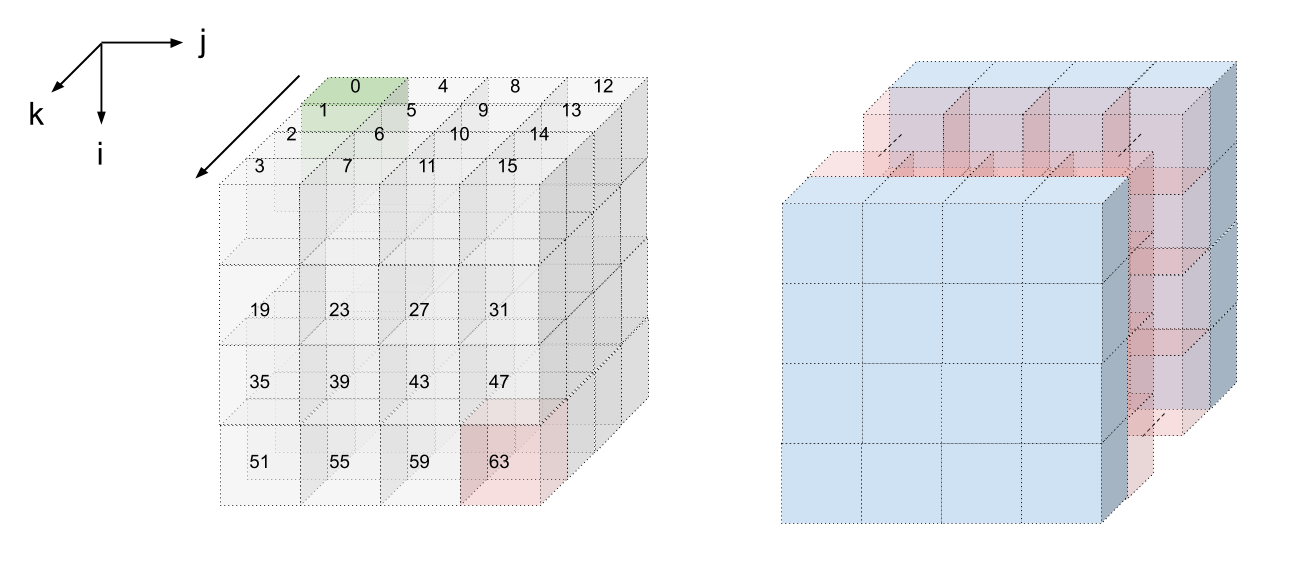
\includegraphics[scale=0.35]{./figures/new/figure_1.png}
  \caption{Illustration of the \texttt{C-order} in files. The left subfigure
  shows how the data is written on disk, with each cube representing a voxel.
  The green block is the first block in the C-order while the red one represents the last block.
  The right subfigure shows how reading or writing only one part of a cuboid written
  in the \texttt{C-order} can produce seeks. Each red voxel is a voxel producing a seek.}
  \label{fig:seeks_and_rowmajor}
\end{figure*}

For the sake of clarity and without loss of generality, we assume that
 files are written in row-major order (Fig~\ref{fig:seeks_and_rowmajor},
 a.k.a ``C" order), where the fastest moving dimension in the file is the
 last dimension of the array, and the slowest moving dimension in the file
 is the first dimension of the array. This convention is for instance the
 one used in the HDF5 format ~\cite{hdf5}. 

Accessing data from an array stored on disk generates seeks in two
situations: (1) when an array block is opened for reading or writing, and (2)
when the reading or writing process moves within the block. 
\tristan{update when figure-right is updated) For a 3D cuboid of shape $C = (C_i, C_j, C_k)$ stored
in row-major order, each column of data in the k dimension is contiguously
stored. There are therefore $C_j \times C_i$ data columns that all require a
seek (see Figure~\ref{fig:seeks_and_rowmajor} (b)).

\subsection{The re-partitioning problem}
We focus on 3D arrays for simplicity. Consider a 3D array of shape $A =
(A_i, A_j, A_k)$, partitioned as evenly-shaped input blocks of shape $I = (I_i,
I_j, I_k)$ stored on disk. Our goal is to re-partition the input blocks into
evenly-shaped output blocks of shape $O = (O_i, O_j, O_k)$, where $O \neq I$.

We formalize the re-partitioning problem as follows.
A re-partioning algorithm (Algorithm~\ref{algo:generalrepartition}) takes a
list of input blocks \texttt{inBlocks} of shape $I$, a list of output
blocks \texttt{outBlocks} of shape $O$, and the amount of memory \texttt{m}
available for the algorithm. Subject to $m$, the algorithm (line 7) determines (1)
\texttt{readBlocks}, a list of evenly-shaped blocks of shape $R$ to be read from the
input blocks, and (2) \texttt{writeBlocks}, a list of blocks,
usually not evenly-shaped, where each block contains a contiuous piece of
data that will be written in an output block with a single seek.
If read blocks and input blocks have a different shape, then reading read blocks requires
more than one seek. Similarly, if write blocks and output blocks have a different shape,
then writing write blocks requires more than one seek. Input, output, read
and write blocks all form a partition of the 3D array of shape $A$. The
main loop of the algorithm (line 9) loads one read block at a time (line
10), inserts it into a cache (line 11), and writes write blocks from the
cache when they are complete (lines 12 to 17).

It should be noted that blocks are passed to the algorithm by reference,
not by data. Only variables \texttt{data} (line 10, 14) and \texttt{cache}
(line 11) hold actual data, contributing to the consumed memory. 

Since read and write blocks both represent a partition of $A$, all the
elements in $I$ are read exactly once, and written exactly once too. Other
problem formalizations may allow for input elements to be read and
discarded, to reduce seeks. Exploring such a trade-off
between seeks and redundant reads could be an interesting extension to this problem.

Our goal is to minimize the number of seeks done by the algorithm, which
occur during reads (line 10) and writes (line 15). We define a cost
function $\mathrm{seeks}$ that returns the number of seeks incurred by the
repartitioning algorithm. 
The re-partitioning problem is therefore to find
the best read and write block lists in order to minimize $\mathrm{seeks}$
subject to the memory constraint $m$. 

% Problem: re-partitioning of multi-dimensional arrays
% Find: readBlocks and writeBlocks 
% Subject to: m
% Such that: seeks is minimal
% \tristan{formalize problem definition}.

Solutions of this problem materialize as implementations of function
\texttt{getReadWriteBlocks} in Algorithm~\ref{algo:generalrepartition}. A
lower bound on the number of seeks for the repartitioning problem is $n_i +
n_o$, with $n_i$ the number of input files and $n_o$ the number of output
files. Indeed, input and output files all have to be accessed at least
once, which requires a seek.

For simplicity, we require that all blocks in \texttt{readBlocks} have
the same shape $R$ \tristan{justify that better}. We also equate the size of an
array in memory as its number of elements.
\tristan{we assume that input and output blocks fit in memory}

\begin{algorithm}
  \caption{General re-partitioning algorithm}
  \label{algo:generalrepartition}
  \begin{algorithmic}[1]
    \STATE \textbf{Inputs}
    \STATE inBlocks: input blocks of shape $I$, stored on disk
    \STATE outBlocks: output blocks of shape $O$, to be written
    \STATE $m$: memory available
    \STATE
    \STATE \textbf{Outputs}
    \STATE none (outBlocks are written)
    \STATE
    \STATE \textbf{Algorithm}
    \STATE readBlocks, writeBlocks $\leftarrow$ getReadWriteBlocks($I$, $O$, $m$)
    \STATE initialize(cache)
    \FOR{readBlock in readBlocks}
      \STATE data $\leftarrow$ read(readBlock, inBlocks)
      \STATE cache.insert(data)
      \FOR{writeBlock in writeBlocks}
        \IF{cache.isComplete(writeBlock)}
          \STATE data $\leftarrow$ cache.pop(writeBlock)
          \STATE write(data, outBlocks)
        \ENDIF
      \ENDFOR
    \ENDFOR

  \end{algorithmic}
\end{algorithm}

\tristan{summarize notations}

\subsection{Algorithms for the split and merge problems}

Special cases of the re-partitioning problem occur when $I=A$ (``split'' problem)
or when $O=A$ (``merge'' problem). Two strategies were introduced
in~\cite{seqalgorithms} to address these problems: the ``multiple" and the
``clustered" strategies. In these strategies, every read block is directly written to the
destination output files, that is, \texttt{readBlocks} and \texttt{writeBlocks} are identical, .
The only difference between the multiple and the clustered strategies lies in
the selection of $R$.

In the split problem studied in~\cite{seqalgorithms} ($I=A$), the naive
strategy defines the read blocks as having the same shape as the output blocks
($R$=$O$). The read blocks are iteratively loaded from $A$ and entirely written
to the appropriate output block (represented by a write block of shape $O$, too).
The "clustered" strategy, however, loads as
many contiguous read blocks of shape $O$ as possible to fit in $m$.
$R$ is therefore a multiple of $O$.
Depending on the amount of main memory available, read blocks may be loaded
individually, by entire block columns, or by entire block slabs.
Although this strategy allows to write each output block in one seek, the clustered strategy is limited by the fact
that it does not optimize the reading step.
In the general re-partitioning problem, one can expect the clustered strategy to
perform poorly as
(1) it reads an output block regardless of its spread among input blocks
and (2) even if it is stored in one input block the algorithm will do a lot of seeks in
case of a shape mismatch \tristan{I dont get (2), to be clarified}.

The "multiple" strategy used for the split problem in~\cite{seqalgorithms}
aims at not doing any seek while reading \textit{and} writing;
Both the input and the output blocks are read/written contiguously. In
terms of Algorithm~\ref{algo:generalrepartition}, it means defining read blocks as
contiguous parts of the input array and write blocks as contiguous parts of
the output arrays. It is equivalent to extending the buffer \tristan{read blocks or write blocks?} in the inverse of
the storage order: $k \rightarrow j \rightarrow i$ in the case
of the \texttt{C-order}. Although the multiple strategy does not seek while reading or writing, it 
requires many switches between output blocks, which also requires seeking. 

To the best of our knowledge, no algorithm has been proposed for the
repartitioning task \tristan{maybe comment more}.

\subsection{Baseline solution}

Our baseline algorithm for the repartitioning problem loads one input block
at a time, that is, $R$=$I$,
and directly writes it to the appropriate output blocks.
The write blocks are therefore defined as the intersections between the input
and output blocks.
For the baseline algorithm, we assume that input block fit in memory ($m \geq I_iI_jI_k$).

The number of seeks $s$ induced by this baseline algorithm is the
sum of the number of seeks done for each read block, that is, the sum of:
\begin{itemize}
  \item the number of input blocks (1 seek per read block)
  \item the number of output blocks openings
  \item the number of seeks done by writing into the output blocks
\end{itemize}

We say that there is a \emph{shape mismatch} in a given dimension $x$ if
input and output blocks are not aligned in dimension $x$. \tristan{make sure that Fig 1 shows i,j,k} A shape mismatch
in dimension $k$, generates $A_iA_j$ seeks in the output blocks, whereas a
shape mismatch in dimension $j$ generates only $A_i$ seeks and a shape
mismatch in dimension $i$ generates a single seek. It should also be noted that if
there are shape mismatches in two dimensions, for instance $k$ and $j$,
then the seeks generated in dimension $j$ are included in the seeks generated
in dimension $k$, resulting in $A_iA_j$ seeks in total. From this
observation we can compute the number of seeks $s$ produced by the naive
strategy as:

\begin{equation} \label{eq:1}
s = A_i A_j c_k + A_i c_j m_k + c_i m_j m_k + N
\end{equation}

With $c_x$ the number of shape mismatches in dimension $x$, $m_x$ is the
number of shape matches in dimension $x$, and $N$ is the number of input blocks. \tristan{why do you need to introduce mx? is it a way to count only the mismatches}.
 The first term corresponds to the seeks produced
by the shape mismatches in $k$, the second term to those in $j$ and the last
term to the mismatches in $i$.

As can be seen in Equation~\ref{eq:1} shape mismatches generate a considerable
 amount of seeks for large arrays $A$. Moreover, a shape mismatch in
 dimension $k$  is more costly than in  dimension $j$, which is itself more
 costly than in dimension $i$ (assuming that the files are stored in
 C-order). For instance, assuming an array of shape $A=(3500, 3500, 3500)$,
 the number of seeks generated by the baseline algorithm is 73,500,000 for a shape mismatch in dimension $k$, 
 147,000 for a shape mismatch in dimension $j$, and 294 for a shape mismatch in dimension $i$.

% We implemented Equation~\ref{eq:1} and ran it on a cubic array to confirm these
% theories. One shape mismatch is added at a time in order to see the impact on
% the number of seeks. The setting and results of this simulation are summarized
% in table~\ref{tab:simseekmodel}.

% \begin{table}[ht]
%   \centering
%   \caption{Results of the simulation using the baseline algorithm's seek model}

%    \begin{tabular}[t]{| c | c | c | c | c |}
%    \hline
%    Mismatch & R & B=I & O & nb seeks \\
%      \hline\hline
%      k & (3500,3500,3500) & (500,500,875) & (500,500,500) & 73,500,000 \\
%      \hline
%      j & (3500,3500,3500) & (500,875,500) & (500,500,500) & 147,000 \\
%      \hline
%      i & (3500,3500,3500) & (875,500,500) & (500,500,500) & 294 \\
%      \hline
%      i,j & (3500,3500,3500) & (875,875,500) & (500,500,500) & 147,168 \\
%      \hline
%      i,j,k & (3500,3500,3500) & (875,875,875) & (500,500,500) & 73,584,096 \\
%      \hline
%    \end{tabular}

%    \label{tab:simseekmodel}

% \end{table}

%----------------------------------------
\section{The \keep heuristic}
%----------------------------------------

\tristan{explain the main idea of the algorithm: brute force, ...}

\subsection{The keep strategy}
As mentioned previously, the baseline, split and merge strategies empty the
cache at each iteration, which generates many seeks in case of a shape
mismatch between the input and output blocks. Instead, the proposed "keep"
strategy aims at maintaining data in the cache when it cannot be written contiguously
to the output blocks (Figure~\ref{fig:keepvsbaseline}).

\begin{figure}[h]
\centering
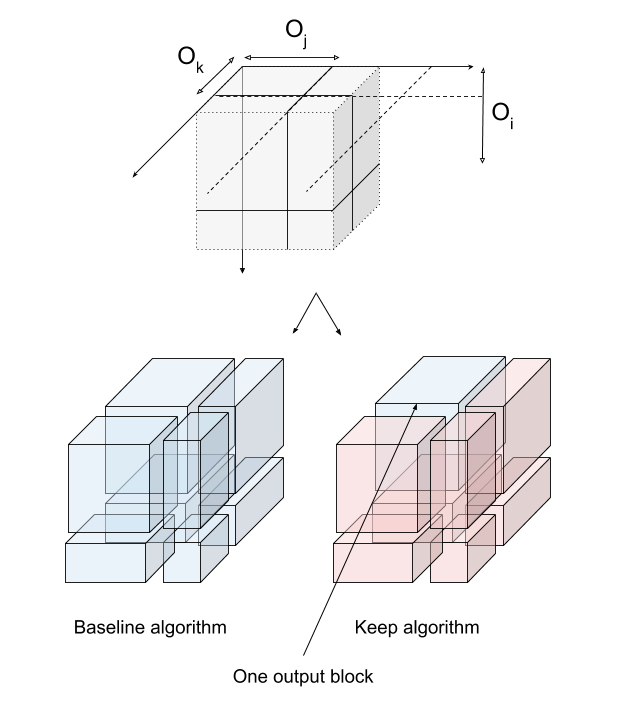
\includegraphics[scale=0.4]{./figures/new/figure_2.png}
\caption{This figure illustrates the difference between the keep and the baseline algorithm.
The first read buffer (on top, grey) is divided in parts by its intersections with output blocks.
While the baseline algorithm writes every part of the read buffer into the appropriate output
blocks (blue cubes are written directly), the keep algorithm writes only the output block
that is complete, and leave the rest in cache until the other parts of the output blocks have been
loaded (red cubes stay in cache). In this figure, $B=\Lambda$.
}
\label{fig:keepvsbaseline}
\end{figure}

\begin{algorithm}
  \caption{Keep heuristic (implements \texttt{getReadWriteBlocks})}
  \label{algo:keep}
  \begin{algorithmic}[1]
    \STATE \textbf{Inputs}
    \STATE inBlocks: input blocks of shape $I$, stored on disk
    \STATE outBlocks: output blocks of shape $O$, to be written
    \STATE $m$: memory available
    \STATE
    \STATE \textbf{Outputs}
    \STATE readBlocks: a list of read blocks
    \STATE writeBlocks: a list of write blocks
    \STATE
    \STATE \textbf{Algorithm}
    \STATE candidates = getCandidateReadShapes($I$, $O$)
    \STATE minSeeks = None
    \FOR{readShape in candidates}
      \STATE writeBlocks = intersection(readBlocks, outBlocks)
      \STATE m' = consumedMemory(readShape, writeBlocks)
      \IF{m' > m}
      \STATE \textbf{continue}
      \ENDIF
      \STATE s' = generatedSeeks(readShape, writeBlocks, $I$, $O$)
      \IF{minSeeks == None or s' < minSeeks}
      \STATE minSeeks, bestReadShape = s', readShape
      \ENDIF
    \ENDFOR
    \STATE writeBlocks = mergeWriteBlocks(writeBlocks, $O$, $m$)
    \STATE readBlocks = blocks(readShape)
    \RETURN readBlocks, writeBlocks
  \end{algorithmic}
\end{algorithm}
The keep heuristic (Alg.~\ref{algo:keep}) implements a brute-force approach
from a list of candidate read shapes (line 11).  
For each candidate read shape, it determines the list of write blocks (line
14),  
the memory consumption of the resulting solution (line 15), and provided that the
memory constraint is repsected, the number of seeks done by the solution (line
19). The read shape leading to the lowest number of seeks is selected (line
20-22). Finally, write blocks are merged as much as allowed by memory constraint (line 24) \tristan{rephrase that when I understand
this part.}, a list of read blocks is generated from the read shape (line
24), and the algorithm returns.

\subsection{Generation of candidate read shapes}

To generate candidate read shapes, we first define a shape $\Lambda$ such
that in each dimension $x$, $\Lambda_x$ is the smallest multiple of $I_x$
that is larger or equal to $O_x$. Using $\Lambda$ as read shape obviously
minimizes the seeks in the input blocks, as in this situation each
iteration reads input blocks completely, requiring 1 seek per input block.
However, seeks are generated when write blocks don't align with output
blocks. \tristan{stopped here}

% # Cas optimal
% # read blocks = Lambda
% # write blocks = output blocks 
% # estime mémoire 

% Si ca fitte pas:
% # read blocks = (1, 1, Lambda_k)
% # write blocks = output blocks inter read buffers

% # Ensuite, étend le read block 
% # Le write block est défini à partir de l'intersection 
% # 


When loading a read block, we call \emph{extra data} the array parts that
are not stored contiguously in the output blocks. The keep strategy
searches for a read block shape $R$ such that $R$ covers at least one
output block completely, i.e., $B_x>O_x$ in all dimensions. It ensures to
always have extra data in case of a shape mismatch, hence making cache
management possible to reduce the number of seeks. We call this ideal read
buffer shape $\Lambda$ \tristan{add to notations / figure}. If $m$ is too
small \tristan{for what?}, then the keep strategy will find a buffer shape
as closed as possible to $\Lambda$. The keep strategy is implemented in
function \texttt{getReadWriteBlocks} called from
Algorithm~\ref{algo:generalrepartition}.

We define the \emph{input aggregate} as the minimum set of input blocks required to 
cover an output block. We call $\Lambda$ the size of the input aggregate. 
For any dimension $x$, if $I_x \geq O_x$, then $\Lambda_x$ is $I_x$. If $I_x < O_x$, then
$\Lambda_x$ is the smallest multiple of $I_x$ which is larger than $O_x$. 


getReadBuffers finds the read block shape $R$ that is the closest to the optimal
shape $\Lambda$, such that $\Lambda_x>O_x$ in any dimension $x$.




If $I_x < O_x$ and there is not enough memory available to ``extend"
the buffer in dimension $x$ such that $R_x > I_x$, then $R_x$ is set to the
largest possible divisor of $A_x$ .

We define an \texttt{input aggregate} as being the minimum aggregate of input
files that covers one output file completely. In particular, $\Lambda$ is the
input aggregate that covers the first output file (indexed $(0,0,0)$) in the
original image being re-partitioned.

\subsection{Searching for the optimal buffer in the inverse storage order}
If $m$ is too small to get $B=\Lambda$, one needs to find in which dimension
the buffer has to be bigger.
For the \texttt{C-order} and given the analysis of the baseline algorithm,
it seems better to have a buffer shape that stores extra data in the $k$
dimension first, rather than in the $j$ or $i$ dimension.
Therefore, if $m$ is too small to get $B=\Lambda$, one must try to get
$B_k=\Lambda_k$ first, then $B_j=\Lambda_j$ and $B_i=\Lambda_i$, i.e. ``extend"
the read buffer in the inverse of the storage order (the storage order being the
C-order here: $i\rightarrow j\rightarrow k$).

In practice, we assume that $m$ is large enough to store a buffer of shape
$(1,1,\Lambda_k)$ which means that we can read one complete data column from an
input block and keep the remainder in memory for the next buffer.
If it was not the case the keep algorithm would not give a significant
improvement in the number of seeks produced by the repartition task, compared
to the baseline algorithm.

\subsection{Consumed memory and generated seeks}

\subsection{Bruteforce search of the read buffer shape}
We found that initializing the buffer to $(1,1,\Lambda_k)$ and stretching the
buffer step by step in the $j$ and then in the $i$ dimension does not reduce
$s$ in a strictly decreasing way which mean we may go over local minima.
We therefore decided to compute the quantity of seeks produced for all the
possible buffers together with their maximum RAM consumption \tristan{how?}.
It is then possible to find the buffer shape producing the less seeks, subject
to $m$.

There is not an infinite possibility for the buffer shapes;
Firstly, the only possibilities for the buffer dimensions are the integer
divisors of R, such that $B_i*B_j*B_k < m$. Indeed, the buffer dimensions must
be integers and the buffer shape B must be a partition of R.
Secondly, as it has been said in the previous subsection, we are only
interested in buffer shapes following the inverse storage order.
It means that we are only interested in buffers that are of the form
$(1,1,R_k)$, $(1,B_j,R_k)$ or $(B_i,R_j,R_k)$ \tristan{unclear}.

\subsection{Impact of the buffer order on performance}
Using the keep strategy, one may order the buffer loadings to reduce the maximum
quantity of extra data stored in memory, hence, reducing the amount of seeks.
For example, if the shape mismatches occur only in the $k$ axis, loading the
buffers in this direction will enable recycling the extra data in cache,
resulting in a smallest memory consumption over time.
The memory saved thanks to a smart
ordering could enable the storage of more extra data in memory using the
keep strategy, further reducing the amount of seeks produced.

As explained in the discussion, the buffer ordering problem is complex and does
not seem easily solvable.
This study uses a naive order which is, again, the inverse storage order.
The reason for that order is that as it is more important to keep data in the
$k$ dimension to save seeks and we assume that $B_k=\Lambda_k$, it seems
reasonable to load the buffers in the $k$ dimension first.
Note that using such
an order recycles extra data in the $k$ dimension first; It is therefore
more efficient when the biggest shape mismatch between the input and output
blocks is in $k$.

Thanksfully, the impact of the buffer ordering on performance can be
mitigated. Indeed, the impact of the buffer ordering depends on the size of the
mismatches. One can reduce the amount of extra data by using smallest blocks: Even
if the overlap between the input and output files is big with respect to their
size, the area/volume of the overlap will be kept small.

\subsection{Remainder volumes}
To compute the maximum RAM consumption of the keep algorithm, given a
buffer shape, we first need to define what a remainder volume is.

A read buffer of shape $\Lambda$ can be divided in
8 parts or ``volumes" (Figure~\ref{fig:nomenclature_overlaps}).
7 out of these 8 volumes are called \texttt{remainder volumes} because
they are created by the shape mismatch between the input files and the output files on
the buffer borders.
The 7 remainder volumes enclose an 8th part that is composed of
input files that are either complete or which complementary part have already
been loaded by a previous buffer. This means that any complementary part is either
in memory (it has been kept in cache according to the keep strategy) or it has
been written down previously.
In other words the remainder volumes contain non contiguous parts of output blocks
as opposed to the non-remainder volume which contains a contiguous part of
an output block.

For read each buffer, each of volume
is indexed following the buffer ordering from $F_0$ to $F_7$, with $F_0$ being the
non-remainder volume. If the buffer is smallest than the input aggregate
($B_x<\Lambda_x$) or if there is no shape mismatch in a given dimension,
it may be that a volume size is set to 0.

\begin{figure*}[h]
\centering
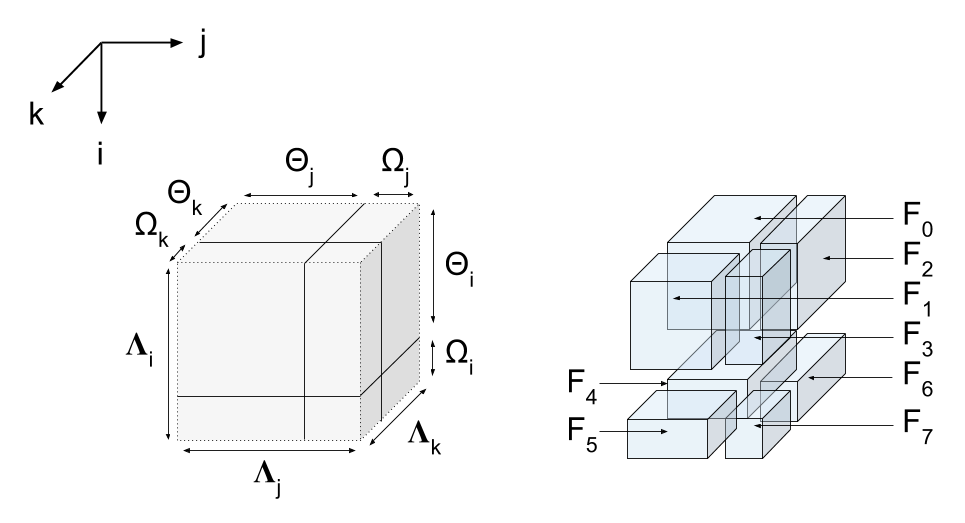
\includegraphics[scale=0.4]{./figures/new/figure_3.png}
\caption{Illustration of an input aggregate (left) and its division into indexed remainder volumes (right).
Each remainder volume is a part of an output block.}
\label{fig:nomenclature_overlaps}
\end{figure*}

\subsection{Maximum memory consumption}
In order to perform the bruteforce search of the best read buffer shape $B$,
we need a way to compute the maximum memory consumption of the algorithm using
this shape.
Having partitioned the buffers into remainder volumes, the maximum memory
consumption can be computed by simulating the re-partition algorithm and
computing, at each step, the cache size.

Let us define $\Sigma$, the amount of data in RAM at a given time during the
execution of the re-partition algorithm.

In order to compute $\Sigma$, the volumes' sizes need to be computed using the
following nomenclature (Figure~\ref{fig:nomenclature_overlaps}):
Given a buffer shape $B$ and the output file shape $O$, we define $C_d(x)$ as
the overlap length between the buffer and an overlaping output file in direction
$d$ for the $x^{th}$ buffer. Let us define $\Omega$ and $\Theta$, that are used
to define upper bounds in the volumes sizes formulas. $\Omega_d(x)$ is the
equivalent of $C_d(x)$ if the buffer was of shape $\Lambda$, and $\Theta_k(x)$
is the difference between $B_d$ and $\Omega_b$, with $B=\Lambda$.
These metrics are computed as follows:
$$C_d(x) = (x+1)B_d mod(O_d)$$
$$\Omega_d(x) = (x+1)\Lambda_d mod(O_d)$$
$$\Theta_d(x) = \Lambda_d - \Omega_d(x)$$

\subsection{Seek estimation for the keep strategy}
In order to compute the amount of seeks produced by the keep algorithm
for a given read shape $B$, we sum of the amount of seeks caused by loading the
read buffers $s_r$ and the amount of seeks caused by writing the write
buffers $s_w$, such that $s=s_r+s_w$.

When loading the read buffers, the seeks occur in case of a shape mismatch
between a read buffer and the input blocks. It is the exact same problem than
when computing the amount of seeks produced by the baseline algorithm when
writing in the output files. Therefore, the baseline seek model presented
before can be used to compute $s_r$.

In order to compute the amount of seeks produced by the write buffers however,
we did not find an elegant formula to solve the problem. We can compute $s_w$
by first finding the write buffers, and then summing the amount of seeks done
by each write buffer. Indeed, given a dimension $x$, a write buffer will seek
if its length in the $x^{th}$ dimension is different than $O_x$.

In particular, with $WB$ the write buffer shape,
\begin{itemize}
  \item $WB_k \neq O_k => WB_i*WB_j$ seeks.
  \item $WB_j \neq O_j => WB_i$ seeks.
  \item $WB_i \neq O_i => 1$ seeks.
\end{itemize}

\subsection{Merging of write blocks}
So far the process to define the read buffers has been described.
getWriteBuffers defines the blocks of data that will be written at once in each
output file.
In the baseline algorithm, the write buffers are defined as the
intersection between the read buffers and the output blocks.
In the context of the keep strategy, some of the remainder volumes are kept in cache
to be written together with other remainder volume(s) contiguously in the output
blocks.
This is equivalent to initializing the write buffers with the same definition as
in the baseline algorithm, and then fusing some of them to be written at once.
The way in which the remainder volumes are fused is summarized in
Table~\ref{tab:fusion}.

\begin{table}[ht]
  \centering
  \caption{Direction(s) in which to fuse the remainder volumes according to the keep strategy, in order to define the write buffers.}

   \begin{tabular}[t]{ | c | c | }
   \hline
   remainder volume's index & direction(s) for the fusion \\
     \hline\hline
     1 & k \\
     \hline
     2 & j \\
     \hline
     3 & j,k \\
     \hline
     4 & i \\
     \hline
     5 & i,k \\
     \hline
     6 & i,j \\
     \hline
     7 & i,j,k \\
     \hline
   \end{tabular}

   \label{tab:fusion}

\end{table}

%----------------------------------------
\section{Implementation}
%----------------------------------------

\subsection{Project repository and programming language}
The baseline algorithm and the ``keep" algorithm have been implemented in plain
Python 3.7.
The Python environment used was a conda environment, all packages used together
with their version are available in a \texttt{requirements.txt} file.
The instructions about how to install the dependencies in a virtual or conda
environement are provided in the \texttt{README} file of the
\href{https://github.com/GTimothee/repartition_experiments}{project's repository}.
The code for all experiments can be found in the same repository as well.

Finally, although we used the HDF5 file format for our experiments, the code
uses an instance of a so-called ``file manager" so that using our code with
another file format is as simple as implementing a new file manager object.

\subsection{Optimizing the main processing loop}
Instead of looping over all write buffers line 15 of
Algorithm~\ref{algo:generalrepartition} we implemented an optimization in
the keep algorithm:
We first compute a Python dictionary associating each buffer to the output files
it crosses or includes.
It allows to search only for the write buffers that write into the output files
crossed by the read buffer loaded. When a write buffer has been written, it
is also deleted from the list of write buffers which reduces even more the
computation time.

\subsection{Optimizing the bruteforce search}
One can note that when the read buffer shape $B$ is smaller than $\Lambda$,
the overall number of buffers increases.
It is therefore quicker to compute the number of seeks and the maximum
quantity of memory to be used for the buffers close to $\Lambda$.
On the contrary, it can take several seconds to compute theses metrics for
small buffers, knowing that among the possible buffer shapes, it is not rare to
see buffers like ($1,1,\Lambda_k$), which is the worst case.
That is why we decided, instead of testing all possible buffer shapes, to start
testing the shapes from the ideal ones ($\Lambda$) to the worst ones
($1,1,\Lambda_k$ for example), reducing the buffer shape in the $j$ dimension
first, and then in $i$.
We only estimate the amount of seeks to be produced if the maximum quantity
to be consumed is smaller than $m$.
We also added a heuristic in order not to test all shapes when it is more
probable that the best shapes are closer to $\Lambda$.
In this spirit, we added a maximum number of iteration above which the search
is stopped if no improvement in the number of seeks has been found.
We set this limit to 10 buffers.

\subsection{Limit to our implementation}
We encountered a tradeoff in the implementation of the keep algorithm which
makes its processing time longer that it could be.
Indeed, we had to implement the keep algorithm by passing data per value from
the read buffers to the cache, instead of by address.
This is due to our formulation of the re-partition problem which requires us to
be able to predict the amount of memory consumed by our algorithm to ensure that
the limit $m$ will be respected.
Python uses a custom garbage collector which manages the release of our
data structures and prevents us to force the release of some data parts.
We found that copying the data to the cache enabled us to stay below the
maximum memory consumption that we predicted at the buffer selection time.

%----------------------------------------
\section{Experiments}
%----------------------------------------

\subsection{Experimental setting}
The experiments have been executed on a private
cluster using \texttt{slurm} as workload manager. Each compute node has 256GB of
RAM, 6 SSDs of size 480 GB and 32 cores. We only used 1 node and 1 SSD at a
time.

\subsection{Comparison of the baseline and the keep algorithms}
In order to assess the keep algorithm performances, we also implemented the
baseline algorithm and ran it in the same conditions than the keep algorithm.
We did one experiment consisting in rechunking an array of shape

$R=(3500,3500,3500)$ and of type \texttt{float16} i.e. with 2 bytes per voxel.
We chose a cubic shape so that no dimension influences more the results than
the other.
Also, the sides of $R$ have been selected to be $3500$ as this number has a
reasonable amount of divisors, which makes the experiment feasible, as
$B$, $O$ and $I$ have to be divisors of $R$.

In this experiment we monitored the processing time of both algorithms, for
different amounts of main memory available.
Indeed, the keep algorithm should be faster when it has more memory available.
In order to test the algorithms in different conditions, we decided to try
several input block shapes, and for each input block shape, two output blocks
shapes have been tested. One output block shape such that $O>I$ and the other
such that $O<I$. This is interesting because when $O>I$ the ideal buffer shape
will be an input aggregate, whereas in the other case $\Lambda=I$.
The different runs have been summarized in Table~\ref{tab:exp} and indexed by
a number.

The three first input blocks have been computed as $R/4$, $R/10$ and $R/20$
(see Table~\ref{tab:exp_inblocks}).
The last input block has a shape of $(350,875,350)$ in order to be of size
approximately 100MB, as recommended by the \texttt{dask} Python package.
With $R/4$, the first input block has a size of about 670MB.
We tried those shapes as they seemed reasonable and can be found in real pipelines.
The only input block shape for which only one output block shape has not been tested
is $R/20$, as using an output block smaller than $R/20$ would be unrealistically
small (about 5.5MB).

The experiment has been run on a cluster node with 256GB, 8GB and 4GB of
available RAM for $m$. \tristan{explain how you reduced the RAM, and the impact on page cache}
The reason for using different amounts of RAM is to benchmark the keep algorithm
with different buffer shapes.
The first amount of RAM corresponds to using all the
available RAM from the compute node, whereas we chose 8 and 4GB of available RAM
because all ideal buffer shapes incured a maximum memory consumption of less than
16GB.
The buffer shapes of each run for each amount of RAM available are summarized in
Table~\ref{tab:buffer_shapes}.

\begin{table}[ht]
  \centering
  \caption{Description of the different runs of the experiment, with $R=(3500,3500,3500)$}

   \begin{tabular}[t]{| c | c | c | c | c |}
   \hline
   $I$ & $O$ & ref \\
   \hline
   \multirow{2}{*}{(875,875,875)} & (875,1750,875) & 0 \\
   & (700,875,700) & 1 \\
   \hline
   \multirow{2}{*}{(350,350,350)} & (500,500,500) & 2 \\
   & (250,250,250) & 3 \\
   \hline
   \multirow{1}{*}{(175,175,175)} & (250,250,250) & 4 \\
   \hline
   \multirow{2}{*}{(350,875,350)} & (500,875,500) & 5 \\
   & (350,500,350) & 6 \\
   \hline
   \end{tabular}

   \label{tab:exp}

\end{table}

\begin{table}[ht]
  \centering
  \caption{Description of the different input block shapes, with $R=(3500,3500,3500)$}

   \begin{tabular}[t]{| c | c | c | c | c |}
   \hline
   $I$ & size (MB) & $R/I$ \\
   \hline
   $(875,875,875)$ & 669.922 & (4,4,4) \\
   \hline
   $(350,350,350)$ & 42.875 & (10,10,10) \\
   \hline
   $(175,175,175)$ & 5.359 & (20,20,20) \\
   \hline
   $(350,875,350)$ & 107.188 & (10,4,10) \\
   \hline
   \end{tabular}

   \label{tab:exp_inblocks}

\end{table}

\begin{table}[ht]
  \centering
  \caption{Description of the different buffer shapes used for each run by the keep algorithm, depending on the amount of RAM available. The last column gives the maximum RAM consumption estimated by the keep algorithm before running (at buffer selection time).}

   \begin{tabular}[t]{| c | c | c | c |}
   \hline
   $m$ & ref & buffer shape & maximum estimated (MB) \\
   \hline
   \multirow{2}{*}{256GB} & 0 & (875, 1750, 875) & 2,679.6875 \\
   & 1 & (875, 875, 875) &  14,631.09375 \\
   & 2 & (700, 700, 700) &  11,596.0 \\
   & 3 & (350, 350, 350) &  5,255.75 \\
   & 4 & (350, 350, 350) &  5,255.75 \\
   & 5 & (700, 875, 700) &  10,920.0 \\
   & 6 & (350, 875, 350) &  1,133.125 \\
   \hline
   \multirow{2}{*}{8GB} & 0 & (875, 1750, 875) & 2,679.6875 \\
   & 1 & (700, 875, 875) &  1,715.0 \\
   & 2 & (500, 700, 700) &  2,040.0 \\
   & 3 & (350, 350, 350) &  5,255.75 \\
   & 4 & (350, 350, 350) &  5,255.75 \\
   & 5 & (500, 875, 700) &  962.5 \\
   & 6 & (350, 875, 350) &  1,133.125 \\
   \hline
   \multirow{2}{*}{4GB} & 0 & (875, 1750, 875) & 2,679.6875 \\
   & 1 & (700, 875, 875) &  1,715.0 \\
   & 2 & (500, 700, 700) &  2,040.0 \\
   & 3 & (250, 350, 350) &  430.0 \\
   & 4 & (250, 350, 350) &  430.0 \\
   & 5 & (500, 875, 700) &  962.5 \\
   & 6 & (350, 875, 350) &  1,133.125 \\
   \hline
   \end{tabular}

   \label{tab:buffer_shapes}

\end{table}

\subsection{Results}

The results in terms of processing times are shown on
Figure~\ref{fig:results}, whereas the results in terms of seeks are
presented on Figure~\ref{fig:seeks_results}.

Looking at Figure~\ref{fig:results}, we can see that
the baseline algorithm performs surprisingly well compared to the keep algorithm
when the main memory available is 256GB (all the node's available RAM).
We can see that when the amount of RAM available decreases (8 and 4GB), the
performances of the baseline algorithm decreases drastically.
In particular, the keep algorithm is approximately 2 times faster for runs
2, 3 and 4 on Figure~\ref{fig:results4}.
From these observations we suppose that the baseline algorithm performs well
with 256GB because it leverages the page cache.
It is counter-intuitive to see that the performances of the baseline algorithm
differs for the different amount of RAM available, because apart from $m$
nothing changes for the baseline algorithm; the read buffer shape stays $B=I$.

Another factor for the baseline algorithm to perform well compared to the
keep algorithm with 256GB is the time overhead of the keep algorithm which is
very important as one can see on Figure~\ref{fig:results}.
This is due to our implementation and the tradeoff presented in section
``Implementation".
Concretely, the time overhead is mainly due to making copies of the data from
the read buffers to the cache.
In terms of read/write processing time however, we can clearly see an
important speedup by the keep algorithm compared to the baseline for
runs 3 and 4 (Figure~\ref{fig:results}).
One can also notice a non-negligible speedup for runs 1 to 5 for the experiment
with 8 (Figure~\ref{fig:results8}) and 4GB (Figure~\ref{fig:results4}).
There are big differences in the benefits of using the keep algorithm instead of
the baseline algorithm, depending on the different runs.
This is due to the difference in complexity between the runs.
The runs that are more complex (with more shape mismatches) are more optimized
by the keep algorithm, hence producing a bigger speedup from the keep compared to
the baseline.

Considering Figure~\ref{fig:seeks_results}, one can see that the number of
seeks is drastically reduced by the keep algorithm, which is consistent with
the results in terms of processing time.
We remark that one needs to reduce significantly the amount of seeks produced
by a re-partition algorithm to clearly see an impact on the processing time.
Considering run 4 which shows the most important differences in terms of
processing time, the amount of seeks have been reduced from about 100 millions
seeks to thousands of seeks.
We also remark that although the number of seeks have been reduced from millions
to thousands of seeks for runs 1 to 5, the reduction in processing time does not
follow linearly the reduction in the number of seeks.
This is probably due to the fact that some seeks are more costly than others,
which has not been taken into account in our problem formulation.

\begin{figure*}
     \centering
     \begin{subfigure}[b]{\textwidth}
         \centering
         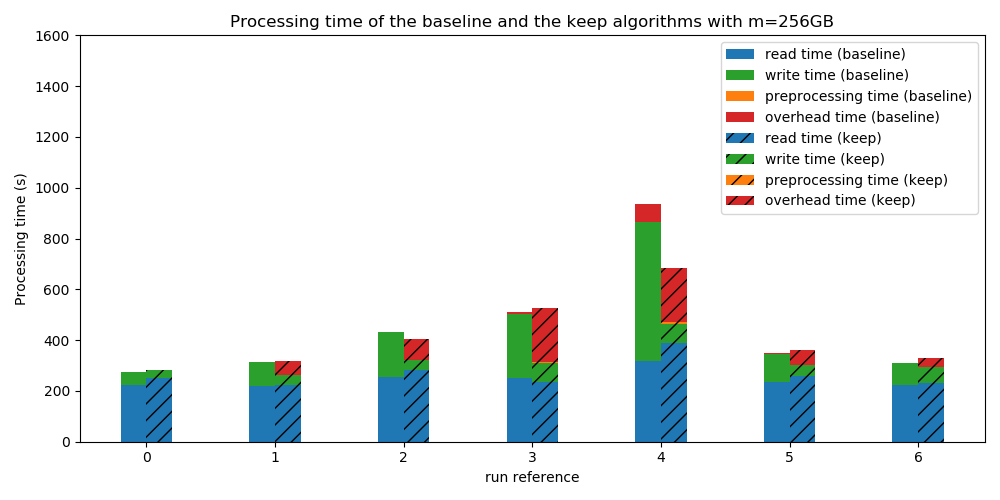
\includegraphics[scale=0.5]{./figures/new/results_256.png}
         \caption{Processing times for $m=256$GB}
         \label{fig:results256}
     \end{subfigure}
     \vfill
     \begin{subfigure}[b]{\textwidth}
         \centering
         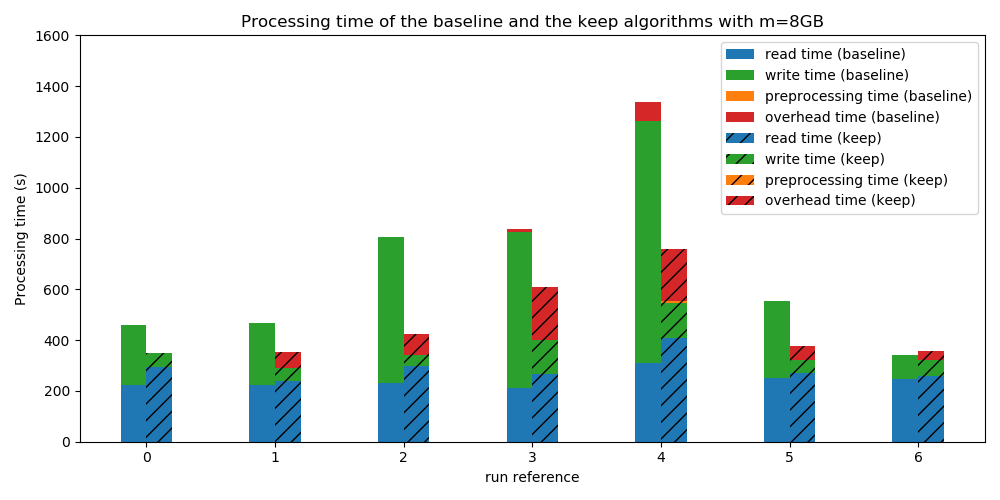
\includegraphics[scale=0.5]{./figures/new/results_8.png}
         \caption{Processing times for $m=8$GB}
         \label{fig:results8}
     \end{subfigure}
     \vfill
     \begin{subfigure}[b]{\textwidth}
         \centering
         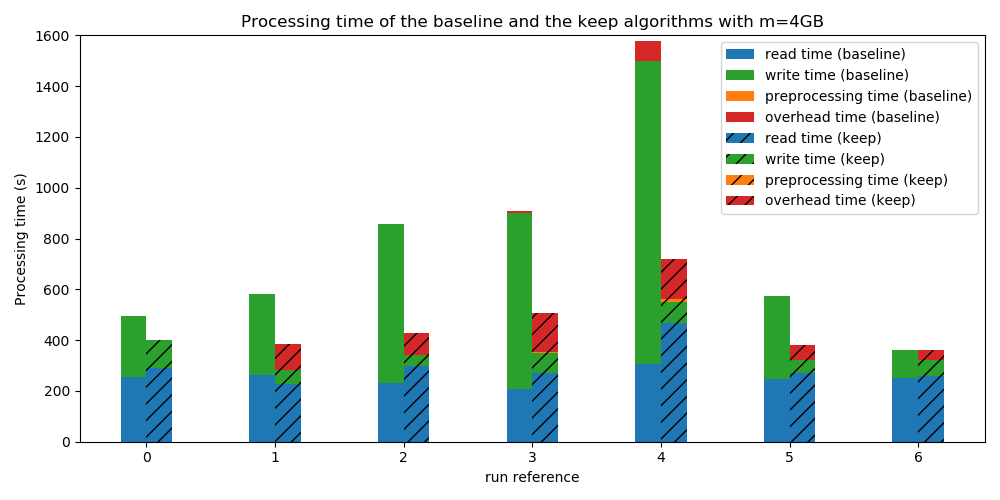
\includegraphics[scale=0.5]{./figures/new/results_4.png}
         \caption{Processing times for $m=4$GB}
         \label{fig:results4}
     \end{subfigure}

     \caption{Results in terms of processing time for the keep and baseline algorithms. From top to bottom, the results are presented for 256, 8 and 4GB of available main memory.}
     \label{fig:results}

\end{figure*}

\begin{figure*}
     \centering
     \begin{subfigure}[b]{\textwidth}
         \centering
         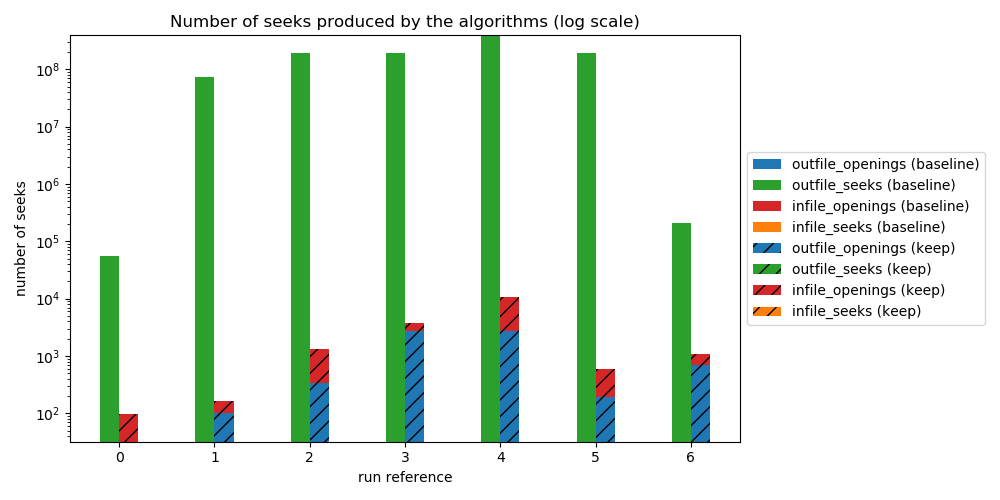
\includegraphics[scale=0.5]{./figures/new/results_seeks_256.png}
         \caption{Seek quantities for $m=256$GB}
         \label{fig:seeks256}
     \end{subfigure}
     \vfill
     \begin{subfigure}[b]{\textwidth}
         \centering
         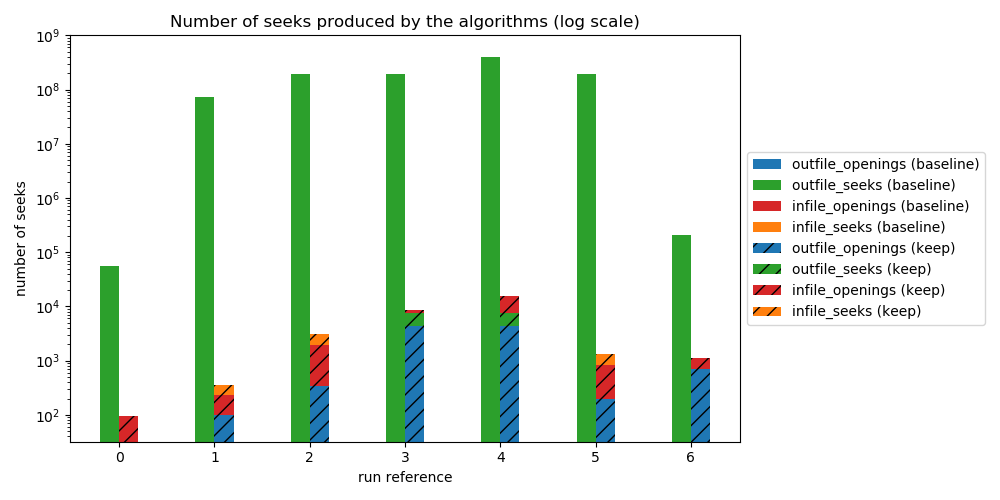
\includegraphics[scale=0.5]{./figures/new/results_seeks_8.png}
         \caption{Seek quantities for $m=8$GB}
         \label{fig:seeks8}
     \end{subfigure}
     \vfill
     \begin{subfigure}[b]{\textwidth}
         \centering
         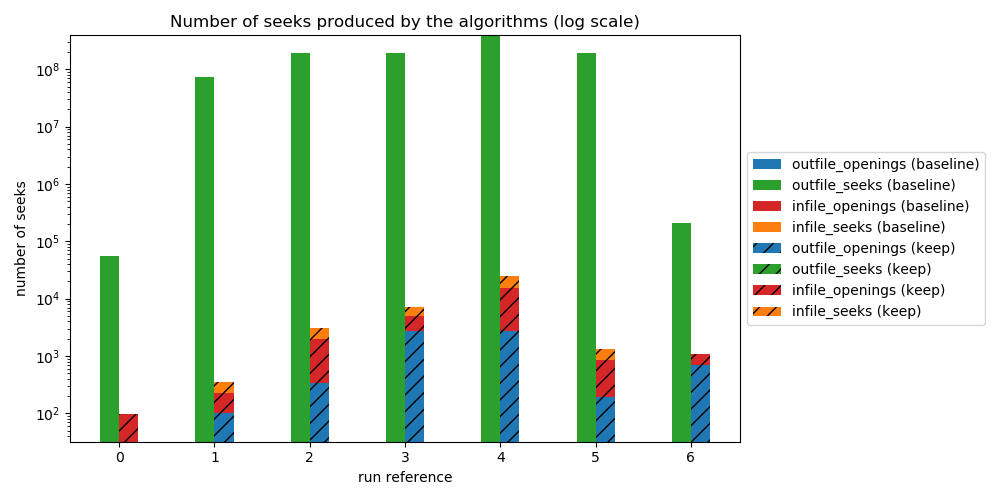
\includegraphics[scale=0.5]{./figures/new/results_seeks_4.png}
         \caption{Seek quantities for $m=4$GB}
         \label{fig:seeks4}
     \end{subfigure}

     \caption{Results in terms of seeks for the keep and baseline algorithms. From top to bottom, the results are presented for 256, 8 and 4GB of available main memory.}
     \label{fig:seeks_results}
\end{figure*}

%----------------------------------------
\section{Discussion}
%----------------------------------------
\tristan{From discussion with Valerie, mention practical considerations related to page cache and readahead}

\subsection{On the keep algorithm}
The keep algorithm can reduce the number of seeks produced by a re-partition
problem from millions to thousands of seeks, compared to the baseline algorithm.
Even if the write time has been drastically reduced on the results shown on
Figure~\ref{fig:results}, there is still margin for improvement in optimizing
the read time.
Finally, it could be interesting to try identifying the type of seeks that are
more costly than the others and focus future implementations of the re-partition
algorithm to reduce such costly seeks.

Although the keep algorithm can be 2 times faster than the baseline algorithm
in some cases, our implementation suffers from a tradeoff between optimizing
the processing time and predicting the maximum amount of memory consumed.
In some non-complex cases, the baseline algorithm can be as efficient as the
keep algorithm.
Moreover, the baseline algorithm seems to take advantage of the surplus of
main memory available in the node, although in theory it is supposed to use
only the size of one input block in bytes at a time.
This does not seem to be the case of the keep algorithm for which the maximum
amount of main memory consumed can be estimated before run.

\subsection{The buffer ordering problem}
The buffer order is important when using the keep strategy, as it defines when
a piece of data will be loaded and when a write buffer will be complete, hence
ready to be written down and freed from the cache.
Representing the read buffers by a complete bidirectional graph in which each
vertex is a buffer, we can model the problem as kind of a complex shortest path
problem.
Indeed, for a given buffer shape $B$, we want to find the read buffers order
that will keep the amount of memory used by the re-partition algorithm low.
Solving this problem would incur more infering at runtime and a potentially
complex algorithm to run.
We decided to keep things simple using a naive buffer order, as the goal of
this study was primarily to assess if the keep algorithm works.

\subsection{ROI extraction problem}
The Region Of Interest (ROI) extraction problem is a related problem that still
needs to be adressed.
A solution using chunking as been introduced in~\cite{optimal_chuking}.
The authors define an array partitioned into chunks of equal shapes and then
define a query as an arbitrary subarray of the input, chunked, array.
They define the optimal chunking problem as finding the optimal chunk such
that the expected number of chunks retrieved to answer the query is minimal.

In our opinion, the solution in~\cite{optimal_chuking} is limited due to the
need of historical or theoretical workload and the necessity to repartition the
input array into an ``optimal" chunk shape.
We would prefer letting the application choose the appropriate chunk shape
regarding its needs and not needing to estimate the processing workload.
We define the ROI extraction problem as follows: Finding an algorithm that takes
as input an arbitrary chunk shape and extract the ROI data from the chunks with
the less number of seeks as possible.

\subsection{Solving three problems at once}
As stated in the introduction, the split and merge tasks are special cases of
the repartition task. This observation leads us to think that maybe one could find
one optimal algorithm for the split, merge and repartition tasks.

If we were to use the keep algorithm with $I=R$, we would read the input data
in slices, exactly like the multiple strategy. The only difference between the
two strategies, however, is that if some remainders appear at the bottom of the
buffer, the keep algorithm would keep it to try to read and write files in one
seek. Not only the keep algorithm tries to limit seeking into the files but it
also tries to limit switching between the files. It would be interesting to
compare the two algorithms for the split/merge tasks to see if the keep
implementation brings similar results or any kind of improvement.

\subsection{The dask Python package}
\texttt{dask} is a popular Python package, part of the SciPy ecosystem, enabling
parallel and out-of-core computations~\cite{matthew_rocklin-proc-scipy-2015}.
It has an important scientific community which is likely to have the problem we
try to solve in this paper, i.e. re-partitioning multidimensional array files.
That is why we would find it interesting to implement our work as an optimization
package for \texttt{dask}.
In particular, we would focus on the \texttt{dask.array} collection, a data
structure designed for multi-dimensional array processing using blocked
algorithms.

\texttt{dask} represents computations as task graphs that are dynamically executed by one
of several schedulers including the single-threaded, the multi-threaded, the
multi-process, and the distributed schedulers. Custom schedulers can also be
implemented. \texttt{dask} graphs can be used out-of-the-box or through
built-in APIs. A \texttt{dask} graph is implemented in plain Python as a
dictionary with any hashable as keys and any object as values. More precisely,
a ``Value" is any object different than a task and a ``Task" is a tuple with a
callable as first element. Examples of APIs/collections include
\texttt{dask.array}, a parallel and out-of-core
Numpy clone, and \texttt{dask.dataframe}, a Pandas clone.
Our first prototype of implementation of the keep algorithm is showing promising
results in optimizing the computation graphs produced by \texttt{dask}.

\subsection{Towards distributed systems}
As most of the big data processing is now done on clusters, it could be interesting
to find distributed versions of the split/merge/re-partition algorithms.
Lots of scientists use HPC (High Performance Computing) clusters regularly which
brings considerations about how to use such distributed algorithms with Lustre
for example, a commonly used filesystem for HPC.

\texttt{dask} also provides a distributed scheduler that seems to be quite
efficient.
It is now recommended for use, even on local computers (using one node).

%----------------------------------------
\section{Conclusion}
%----------------------------------------

Multidimensional array chunking is a routine for scientists nowadays.
That is why efficiently processing such arrays is of major importance in the big data era.

Splitting and merging arrays has been successfully done, we therefore attempted
to solve the next step: the re-partitioning problem.
This problem consists in efficiently re-writing a chunked array to change the blocks shape.
We think that solving this problem could enable us to solve the ROI (region of interest)
extraction problem in the future, which is also a very common problem for scientists.
We formally defined the re-partitioning problem together with a \emph{baseline algorithm} to solve it.
We also presented the \emph{keep algorithm} to reduce the number of seeks produced during
the re-partitioning and hopefully reduce the processing time of such task.
The keep algorithm reduces the number of seeks by
(1) constraining the read buffers shape to minimize the read time, and
(2) leveraging a ``cache" to minimize the write time.

Although the re-partitioning problem is more complex than splitting/merging chunks,
we proved that it can be optimized and that it is possible to reduce the
processing time significantly.
Surprisingly however, the baseline algorithm has been found to perform pretty
well when there is a lot of memory available as it leverages the page cache to
speedup computations without reducing the number of seeks.
For now, the keep algorithm may be more interesting than the baseline algorithm
only when the memory constraint is important ($m$ small compared to the array size).

In the future, the algorithm performances may be improved by finding a variant
to the keep algorithm that also reduce the read time significantly,
identifying and focusing on reducing the most expensive seeks,
and finally, finding parrallel and/or distributive versions of the keep algorithm.

%----------------------------------------
\section{Acknowledgments}
%----------------------------------------

The computing platform was obtained with funding from the Canada Foundation for Innovation.

\tristan{Timothée, make sure that all references have a title, date, and venue (journal or conference name). 
Check capitalization of words like HDF5, etc}

\bibliography{Bibliography}
\bibliographystyle{ieeetr}

\end{document}
